%
% Analysis
%
\chapter{Preliminary Experiments} \label{sec:preliminary}
In this chapter we perform preliminary experiments to investigate the effects of non-stationarity and the transferability of RL agents in VGC.
The goal of these experiments is to answer the following questions:

\begin{enumerate}
    \item What effect does non-stationarity have on the performance and generalization of reinforcement learning agents in VGC?
    \item To what extent are reinforcement learning agents able to maintain performance under non-stationarity without any continual learning techniques?
\end{enumerate}

We first formalize our problem statement outlined in Chapter \ref{sec:introduction}:
Let $A_t$ be an agent that is trained from scratch on a unique version $t$ of a two-player zero-sum game $\mathcal{G}_t$ for $n$ steps.
Our goal is to identify or propose training paradigms that allow $A_t$ to outperform (i.e. have a higher win rate than) agent $A_{t+1}$ on $\mathcal{G}_{t+1}$, in at most $n$ additional training steps.
Additionally, we make the following assumptions:

\begin{assumption} \label{ass:increasing}
    $t$ is monotonically increasing.
\end{assumption}

\begin{assumption} \label{ass:task}
    $\mathcal{G}_{t+1}$ has the same action space and reward function as $\mathcal{G}_{t}$.
\end{assumption}

\begin{assumption} \label{ass:availability}
    Knowledge about $\mathcal{G}_{t+1}$ is unavailable when training on $\mathcal{G}_{t}$.
\end{assumption}

For VGC, this amounts to agent $A_0$ being trained on regulation \textbf{A}, after which it will have to transfer its learned knowledge to regulation \textbf{B}, then to regulation \textbf{C}, etc.
Under assumption \ref{ass:increasing}, no regulation will be revisited after it is played.
Under assumption \ref{ass:task}, we can classify this problem as a \textit{domain-incremental learning} problem, where agents have to adapt to a non-stationary input distribution (different teams in different regulations).

As discussed in Chapter \ref{sec:vgc:vgc-bench}, VGC-Bench provides six different RL agents that could serve as the basis for experiments in this thesis.
Although the fine-tuned behavior cloning agents show the best results, the behavior cloning model is trained on trajectories of all regulations~\cite{angliss2025vgc}.
Consequently, choosing any of the three fine-tuned behavior cloning agents would violate assumption \ref{ass:availability}.
Out of the remaining three RL agents, we opt for the \textit{regular self-play} model, because of its well-established position in the literature.

Another important parameter for training agents using VGC-Bench is the number of teams in an agent's in-distribution set (the number of teams the agent sees during training).
\textcite{angliss2025vgc} consider a variety of numbers of teams seen during training, ranging from just one team up to 64 unique teams per regulation.
Their findings show that, although larger in-distribution sets lead to worse overall performance, they do lead to significantly better generalization to out-of-distribution teams~\cite{angliss2025vgc}.
Additionally, a larger in-distribution set also decreases the variance caused by how this set is sampled from the pool of all available teams.
Since regulations define which teams can be sampled into the in-distribution set, we speculate that agents trained with a larger in-distribution set can generalize better to different regulations than agents trained with a smaller in-distribution set.
For this reason, we train all agents using the largest number of teams considered by \textcite{angliss2025vgc}: 64 unique teams per regulation.

\section{Zero-Shot Transfer} \label{sec:preliminary:transfer}
To establish to what extent non-stationarity harms the performance of RL agents, we investigate whether RL agents trained on different regulations are capable of zero-shot transfer to other regulations.
We train 10 RL agents using regular self-play, one on each of the 10 regulations shown in Table \ref{tab:regulations}, using the same hyperparameters as VGC-Bench (shown in Table \ref{tab:hyperparam-vgcbench}).
We evaluate by running 1000 episodes of cross-play between all agents in every regulation. The results of this experiment can be found in Figure \ref{fig:zeroshot-indist}.

\begin{figure}[ht]
    \centering
    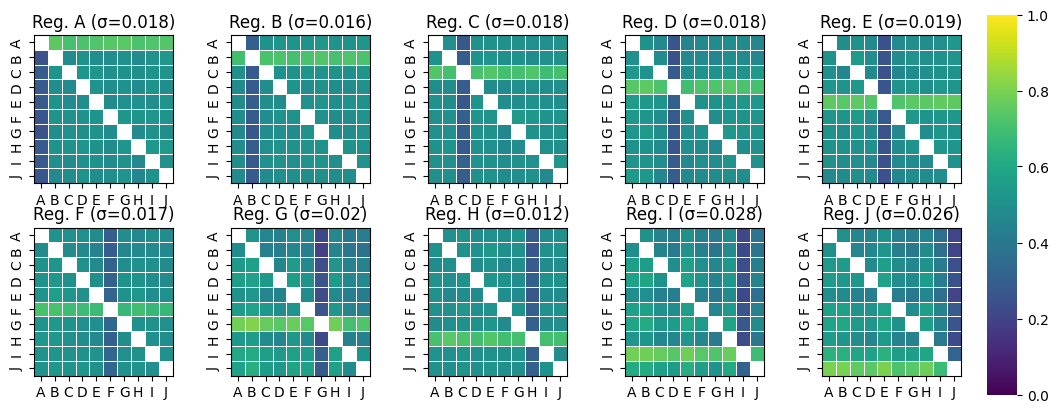
\includegraphics[width=\textwidth]{images/preliminary/zero-shot-in-dist.png}
    \caption{Win rates of the row player over 1000 episodes and three seeds, evaluated in-distribution on each regulation. Letters on the axes represent the regulation the agent is trained on. More in-depth figures for every regulation can be found in Appendix \ref{app:figures}.}
    \label{fig:zeroshot-indist}
\end{figure}

We can observe in Figure \ref{fig:zeroshot-indist} that every agent can consistently win in the regulation that they are trained on, though it should be noted that the teams used for cross-play are all sampled from the in-distribution set of the agent trained on the regulation, potentially biasing the results in favor of that agent.
To evaluate the generalization of the agents to unseen teams, we run a second cross-play experiment using the out-of-distribution set of the agent trained on the regulation, meaning none of the teams have been seen by any agent before.
The results of this experiment can be found in Figure \ref{fig:zeroshot-outofdist} (note that regulations \textbf{B}, \textbf{E}, and \textbf{J} are excluded because there are not enough teams available for a full out-of-distribution set).

\begin{figure}[H]
    \centering
    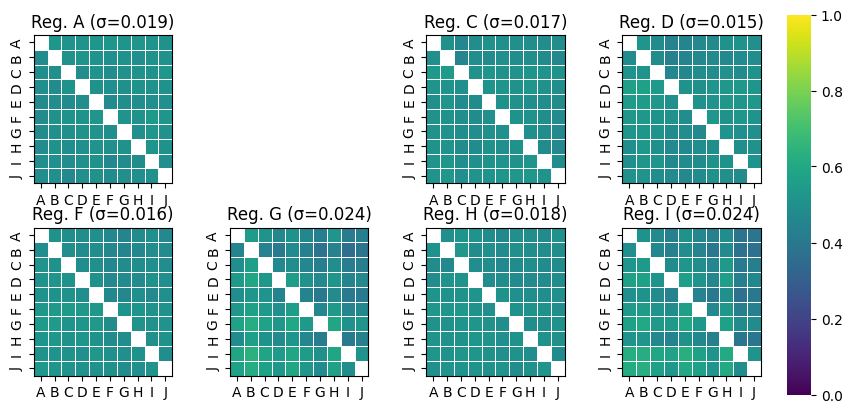
\includegraphics[width=0.85\textwidth]{images/preliminary/zero-shot-out-of-dist.png}
    \caption{Win rates of the row player over 1000 episodes and three seeds, evaluated out-of-distribution on each regulation (excluding regulations \textbf{B}, \textbf{E}, and \textbf{J}). Letters on the axes represent the regulation the agent is trained on. More in-depth figures can be found in Appendix \ref{app:figures}.}
    \label{fig:zeroshot-outofdist}
\end{figure}

We can observe in Figure \ref{fig:zeroshot-outofdist} that the out-of-distribution results are a lot less clear than the in-distribution results shown in Figure \ref{fig:zeroshot-indist}, but, especially in later regulations, there appears to still be an advantage for the agents trained in the same regulation that the cross-play is performed in.

To verify our results, we define our null hypothesis $H_0$ to be that an agent trained on regulation $t$ performs worse than an agent trained on any regulation $\tau \neq t$ when playing in regulation $t$.
We define our significance level to be $\alpha=0.05$.
We can use a Binomial test with $n=1000$ and an expected win rate of $p < 0.5$ to calculate the p-values of the win rates of each row player in the regulation they are trained on.
These p-values are shown in Figure \ref{fig:zeroshot-pvalues}.

\begin{figure}[ht]
    \centering
    \begin{subfigure}{.4\textwidth}
        \centering
        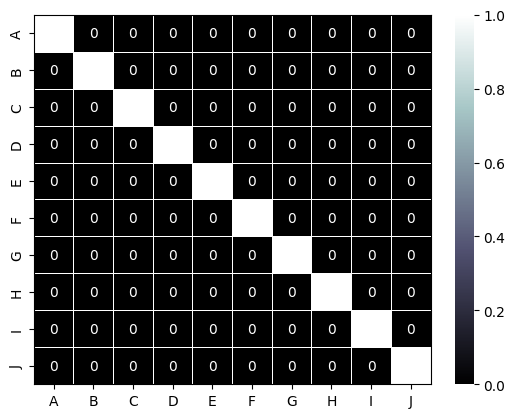
\includegraphics[width=\textwidth]{images/preliminary/zero-shot-in-dist-pvalues.png}
        \caption{In-distribution.}
        \label{fig:zeroshot-pvalues-indist}
    \end{subfigure}
    \hfill
    \begin{subfigure}{.5\textwidth}
        \centering
        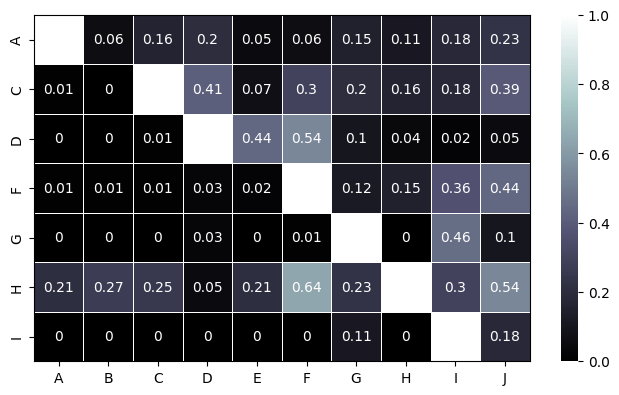
\includegraphics[width=\textwidth]{images/preliminary/zero-shot-out-of-dist-pvalues.png}
        \caption{Out-of-distribution.}
        \label{fig:zeroshot-pvalues-outofdist}
    \end{subfigure}
    \caption{P-values of the win rates of the row player in the regulation that they are trained on. Letters on the axes represent the regulation the agent is trained on.}
    \label{fig:zeroshot-pvalues}
\end{figure}

Observe that all p-values are smaller than 0.05 in Figure \ref{fig:zeroshot-pvalues-indist}, meaning we can reject $H_0$ and conclude that the result for in-distribution cross-play is statistically significant: RL agents are not capable of zero-shot transfer to different regulations.
For Figure \ref{fig:zeroshot-pvalues-outofdist}, things are more complicated.
We can see a general trend emerge that p-values are smaller than 0.05 when agents are evaluated against agents trained on a previous regulation, but larger than 0.05 when evaluated against agents trained on a future regulation, though both of these trends do have exceptions.
We suspect this may be because of the superset relation between different regulations, which would also explain why regulation \textbf{H} seems to be an exception to the general trend.

For the out-of-distribution cross-play results, we can tentatively reject $H_0$ for cases where an agent plays against an agent trained on a previous regulation, and tentatively retain $H_0$ for cases where an agent plays against an agent trained on a future regulation.
This means that, generally speaking, RL agents are capable of zero-shot transfer to future regulations when neither agent has seen the teams before, but incapable of zero-shot transfer in any other scenario.

\section{Full Fine-Tuning} \label{sec:preliminary:finetune}
To establish to what extent RL agents can maintain performance under non-stationarity without using any continual learning techniques, we investigate whether we can transfer the agents trained in Chapter \ref{sec:preliminary:transfer} to other regulations using full fine-tuning.

Staying in line with the problem statement defined at the beginning of this chapter, we start with an agent trained on regulation \textbf{A}.
This agent is then fine-tuned to regulation \textbf{B}, then to regulation \textbf{C}, etc.
Fine-tuning is always done for the same number of steps and using the same hyperparameters as regular training (shown in Table \ref{tab:hyperparam-vgcbench}) to provide an upper bound of the expected performance.
After fine-tuning on a regulation, we evaluate the fine-tuned agent by having it play an agent trained from scratch in that regulation for 1000 episodes.
The results for this experiment can be found in Figure \ref{fig:finetune}.

\begin{figure}[ht]
    \centering
    \begin{subfigure}{.5\textwidth}
        \centering
        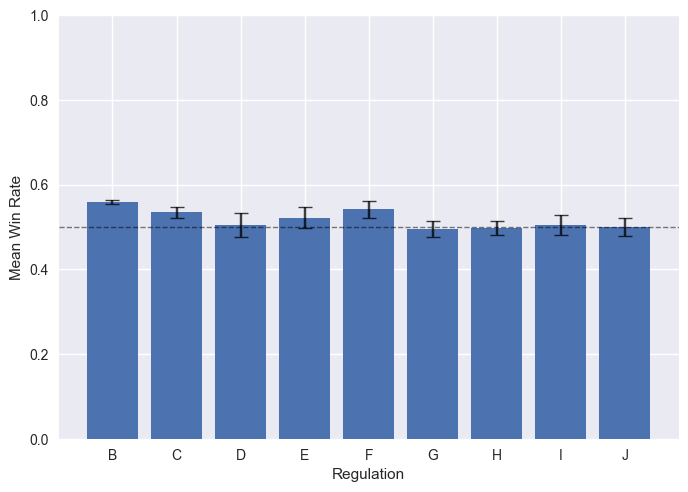
\includegraphics[width=\textwidth]{images/preliminary/finetune-in-dist.png}
        \caption{In-distribution.}
        \label{fig:finetune-indist}
    \end{subfigure}%
    \begin{subfigure}{.5\textwidth}
        \centering
        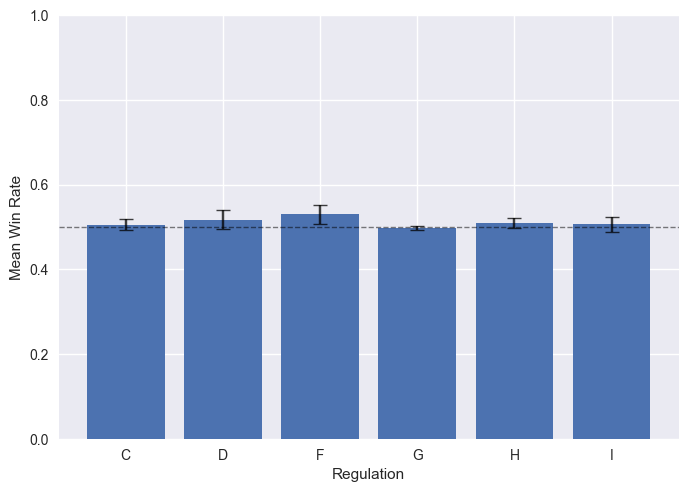
\includegraphics[width=\textwidth]{images/preliminary/finetune-out-of-dist.png}
        \caption{Out-of-distribution.}
        \label{fig:finetune-outofdist}
    \end{subfigure}
    \caption{Mean win rates of fine-tuned agents against agents trained from scratch. Evaluated over 1000 episodes and three seeds on each regulation. More in-depth figures can be found in Appendix \ref{app:figures}.}
    \label{fig:finetune}
\end{figure}

To verify these results, we define our null hypothesis $H_0$ to be that an agent $\phi$ is equally skilled or worse than an agent $\psi$, and we define our significance level to be $\alpha=0.05$.
We can use a Binomial test with $n=1000$ and an expected win rate of $p \leq 0.5$ to calculate the p-values of the win rates of agent $\phi$.
These p-values can be found in Figure \ref{fig:finetune-pvalues}.

\begin{figure}[H]
    \centering
    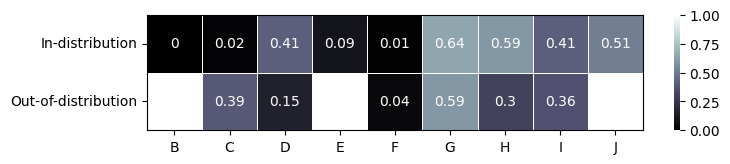
\includegraphics[width=\textwidth]{images/preliminary/finetune-pvalues.png}
    \caption{P-values of the mean win rates of fine-tuned agents against agents trained from scratch. Letters on the horizontal axis represent the regulation the agents are trained or fine-tuned on.}
    \label{fig:finetune-pvalues}
\end{figure}

The results shown in Figures \ref{fig:finetune} and \ref{fig:finetune-pvalues} are quite mixed.
While there are cases where we see an agent experience positive transfer and beat an agent trained from scratch (particularly in the earlier regulations and when evaluating using in-distribution teams), $H_0$ is retained for the majority of cases.
This leads us to tentatively conclude that, in the best case, positive transfer without continual learning is possible short-term, but becomes harder as the non-stationarity increases over time.

\section{Further Analysis} \label{sec:preliminary:analysis}
One trend visible in Figure \ref{fig:finetune} is that the positive transfer is clearly visible in regulation \textbf{F}, but starts to collapse in regulation \textbf{G}, both in-distribution and out-of-distribution.
We decide to analyze these two cases more closely, as any insights gained here could potentially help us prolong the positive transfer using continual learning.

To gather more data about these two cases, we run 100 additional episodes of cross-play on regulations \textbf{F} and \textbf{G}, both in-distribution and out-of-distribution, collecting statistics such as action probabilities, action logits, and value predictions for every observation from three agents: The agent trained on the regulation from scratch, the agent fine-tuned up to the regulation, and the agent fine-tuned up to the previous regulation (the source agent of the other fine-tuned agent).

Our first experiment focuses on the similarity between the action probabilities, which should show us how similar the agents are in their decision making when given the same observation.
We use the Jensen-Shannon (JS) distance, a symmetric version of the Kullback-Leibler (KL) divergence that is bounded to $[0,1]$ (lower values indicating more similar probability distributions), to calculate the distance between two action probability distributions~\cite{dagan1997jsdistance}.
These results, plotted against the normalized depth of the observation (how many turns into the battle it was recorded), can be found in Figure \ref{fig:jsd}.

\begin{figure}[H]
    \centering
    \begin{subfigure}{.5\textwidth}
        \centering
        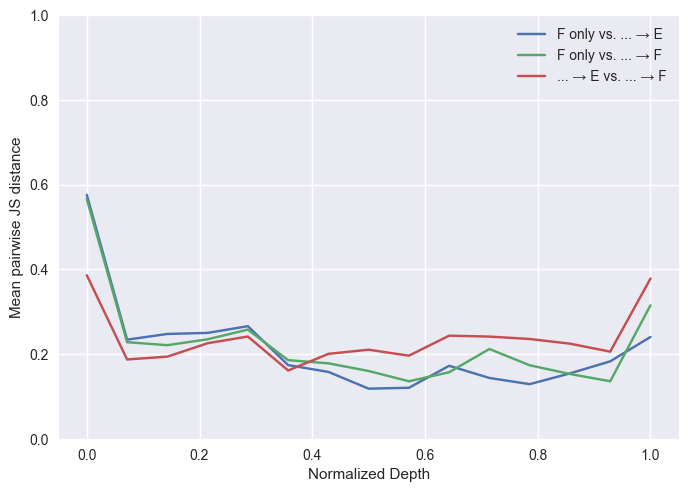
\includegraphics[width=\textwidth]{images/preliminary/jsd-depth-regf-indist.png}
        \caption{Regulation \textbf{F}, in-distribution ($n=974$).}
        \label{fig:jsd-regf-indist}
    \end{subfigure}%
    \begin{subfigure}{.5\textwidth}
        \centering
        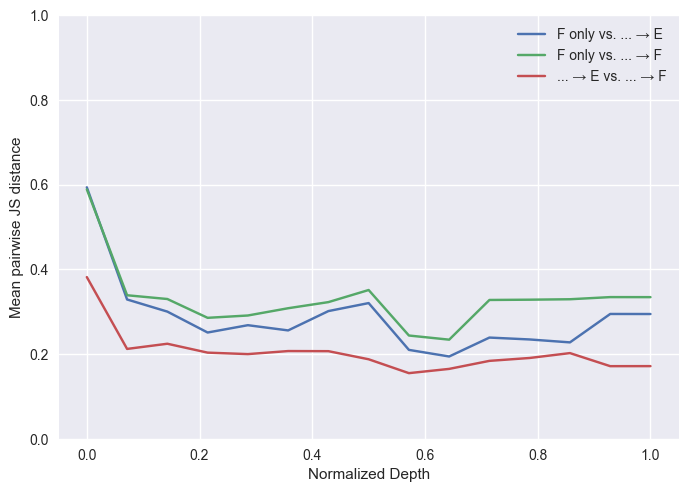
\includegraphics[width=\textwidth]{images/preliminary/jsd-depth-regf-outofdist.png}
        \caption{Regulation \textbf{F}, out-of-distribution ($n=1035$).}
        \label{fig:jsd-regf-outdist}
    \end{subfigure}
    \vskip\baselineskip
    \begin{subfigure}{.5\textwidth}
        \centering
        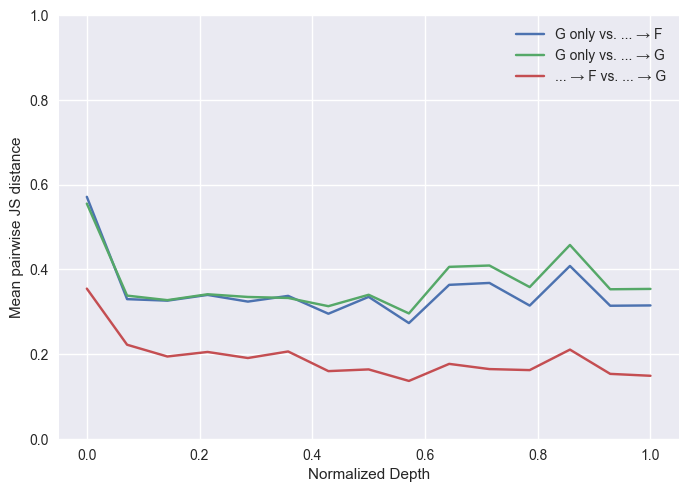
\includegraphics[width=\textwidth]{images/preliminary/jsd-depth-regg-indist.png}
        \caption{Regulation \textbf{G}, in-distribution ($n=1086$).}
        \label{fig:jsd-regg-indist}
    \end{subfigure}%
    \begin{subfigure}{.5\textwidth}
        \centering
        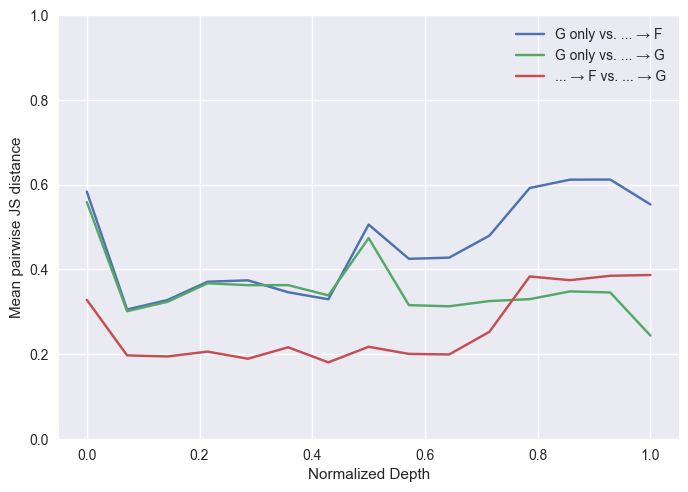
\includegraphics[width=\textwidth]{images/preliminary/jsd-depth-regg-outofdist.png}
        \caption{Regulation \textbf{G}, out-of-distribution ($n=1101$).}
        \label{fig:jsd-regg-outdist}
    \end{subfigure}
    \caption{Mean pairwise Jensen-Shannon distance between action probabilities for every observation, plotted against the normalized depth. Letters represent the regulation the agent is trained or fine-tuned on (e.g. ``$... \rightarrow \text{F}$" is fine-tuned from regulation \textbf{A} to \textbf{B} to ... to \textbf{F}).}
    \label{fig:jsd}
\end{figure}

Starting with the in-distribution results shown in Figures \ref{fig:jsd-regf-indist} and \ref{fig:jsd-regg-indist}, we can observe that the distance between the action probabilities of the two fine-tuned models (the red line) is consistently below the distance between the fine-tuned models and the model trained from scratch (the blue and green lines) for regulation \textbf{G}, while the three lines appear more balanced for regulation \textbf{F}.
Intuitively, this points towards a potential loss of plasticity in regulation \textbf{G}, keeping the fine-tuned model too similar in behavior to its source model and preventing it from fully adapting to regulation \textbf{G}.

Moving to the out-of-distribution results in Figures \ref{fig:jsd-regf-outdist} and \ref{fig:jsd-regg-outdist}, we can observe a similar trend in regulation \textbf{F} this time, although the differences are clearly smaller here.
In regulation \textbf{G} we can see a big shift compared to the other figures, especially for deeper observations.
While the red line stays below the other lines for most of the observations, we actually see the distance between the fine-tuned model and the model trained from scratch go below it near the end, suggesting that there is no loss of plasticity here.
This mixed result makes it difficult to draw concrete conclusions from this experiment.

In the next experiment we compare the value predictions of the agents when given the same observation.
We showed in Chapter \ref{sec:preliminary:finetune} that these agents have close to a 50\% win rate against each other, suggesting that we should expect to see value predictions centered around zero.
The results for this experiment, plotted against the normalized depth of the observation, can be found in Figure \ref{fig:value}.

\begin{figure}[H]
    \centering
    \begin{subfigure}{.5\textwidth}
        \centering
        
\includegraphics[width=\textwidth]{images/preliminary/value-regf-indist.png}
        \caption{Regulation \textbf{F}, in-distribution ($n=974$).}
        \label{fig:value-regf-indist}
    \end{subfigure}%
    \begin{subfigure}{.5\textwidth}
        \centering
        
\includegraphics[width=\textwidth]{images/preliminary/value-regf-outofdist.png}
        \caption{Regulation \textbf{F}, out-of-distribution ($n=1035$).}
        \label{fig:value-regf-outdist}
    \end{subfigure}
    \vskip\baselineskip
    \begin{subfigure}{.5\textwidth}
        \centering
        
\includegraphics[width=\textwidth]{images/preliminary/value-regg-indist.png}
        \caption{Regulation \textbf{G}, in-distribution ($n=1086$).}
        \label{fig:value-regg-indist}
    \end{subfigure}%
    \begin{subfigure}{.5\textwidth}
        \centering
        
\includegraphics[width=\textwidth]{images/preliminary/value-regg-outofdist.png}
        \caption{Regulation \textbf{G}, out-of-distribution ($n=1101$).}
        \label{fig:value-regg-outdist}
    \end{subfigure}
    \caption{Mean value prediction for every observation, plotted against the normalized depth. Letters represent the regulation the agent is trained or fine-tuned on (e.g. ``$... \rightarrow \text{F}$" is fine-tuned from regulation \textbf{A} to \textbf{B} to ... to \textbf{F}).}
    \label{fig:value}
\end{figure}

We can see in Figure \ref{fig:value} that the value predictions clearly do not fit our expectation of being centered around zero, instead showing quite unstable and inconsistent behavior.
The predictions shown in Figures \ref{fig:value-regf-indist}, \ref{fig:value-regf-outdist}, and \ref{fig:value-regg-outdist} show quite severe jumps, and in Figure \ref{fig:value-regf-indist} the mean value prediction of the model fine-tuned up to regulation \textbf{E} even drops below the minimum reward of -1 at some point.
These unexpected results make it difficult to conclude anything meaningful with regards to the transfer process, though there is an argument to be made that the value predictions of the model trained from scratch shows the least extreme behavior.
These results mainly raise further questions about the cause of these unstable value predictions, and their potential effect on the overall performance and transferability of the model.

The last experiment in this chapter involves the action logits computed by the agents.
We are interested in whether we can gain further insights into the transfer process by plotting the distribution of action logits using a t-SNE visualization.
We take the 256-dimensional action logits for each observation, reduce them to 50 dimensions using principal component analysis (PCA), then reduce them to two dimensions using t-SNE~\cite{van2008tsne}.
These visualizations can be found in Figure \ref{fig:tsne}.

\begin{figure}[H]
    \centering
    \begin{subfigure}{.5\textwidth}
        \centering
        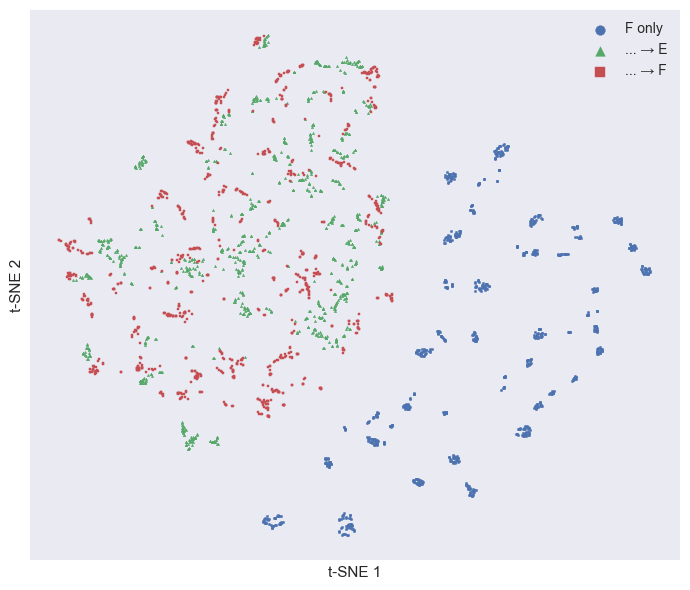
\includegraphics[width=\textwidth]{images/preliminary/tsne-regf-indist.png}
        \caption{Regulation \textbf{F}, in-distribution ($n=974$).}
        \label{fig:tsne-regf-indist}
    \end{subfigure}%
    \begin{subfigure}{.5\textwidth}
        \centering
        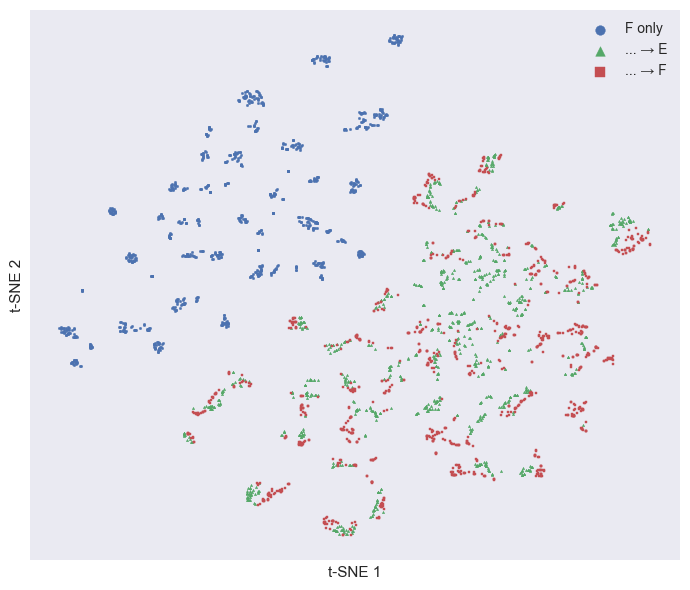
\includegraphics[width=\textwidth]{images/preliminary/tsne-regf-outofdist.png}
        \caption{Regulation \textbf{F}, out-of-distribution ($n=1035$).}
        \label{fig:tsne-regf-outdist}
    \end{subfigure}
    \vskip\baselineskip
    \begin{subfigure}{.5\textwidth}
        \centering
        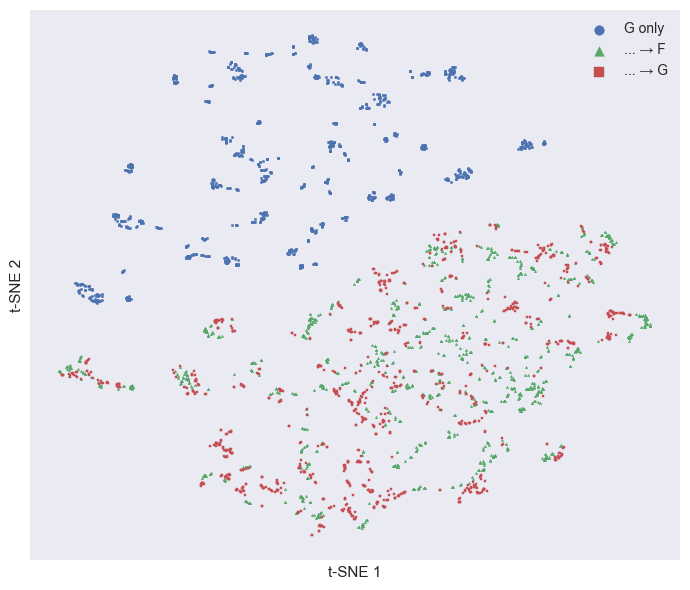
\includegraphics[width=\textwidth]{images/preliminary/tsne-regg-indist.png}
        \caption{Regulation \textbf{G}, in-distribution ($n=1086$).}
        \label{fig:tsne-regg-indist}
    \end{subfigure}%
    \begin{subfigure}{.5\textwidth}
        \centering
        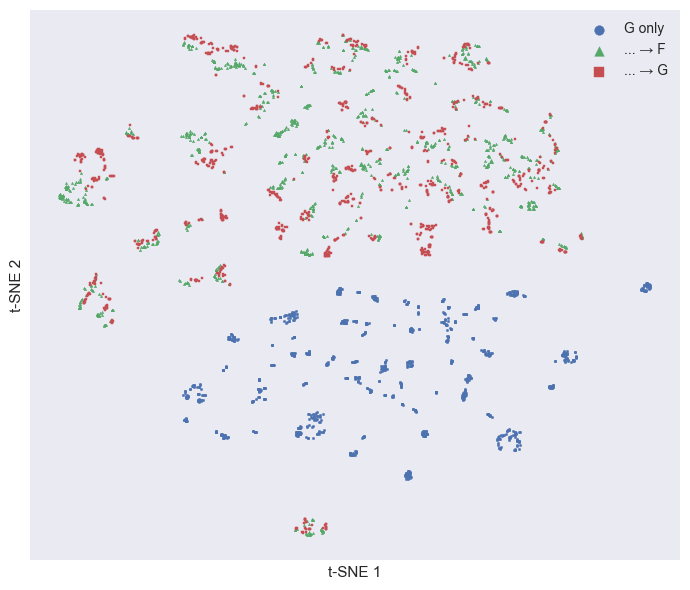
\includegraphics[width=\textwidth]{images/preliminary/tsne-regg-outofdist.png}
        \caption{Regulation \textbf{G}, out-of-distribution ($n=1101$).}
        \label{fig:tsne-regg-outdist}
    \end{subfigure}
    \caption{t-SNE visualization of action logits for every observation. Letters represent the regulation the agent is trained or fine-tuned on (e.g. ``$... \rightarrow \text{F}$" is fine-tuned from regulation \textbf{A} to \textbf{B} to ... to \textbf{F}).}
    \label{fig:tsne}
\end{figure}

A trend visible in Figure \ref{fig:tsne} is that the action logits of the model trained from scratch (the blue circles) appear to be distinguishable from the action logits of the models that are fine-tuned.
To get a clearer picture of the underlying structure, we sample 50 observations (150 points) from the above figures and connect points showing logits of the same observations.
Since t-SNE distorts global and local distances, we color these connecting lines according to the Jensen-Shannon distance between the action probabilities of the respective observations.
These visualizations can be found in Figure \ref{fig:tsne-lines}.

\begin{figure}[H]
    \centering
    \begin{subfigure}{.5\textwidth}
        \centering
        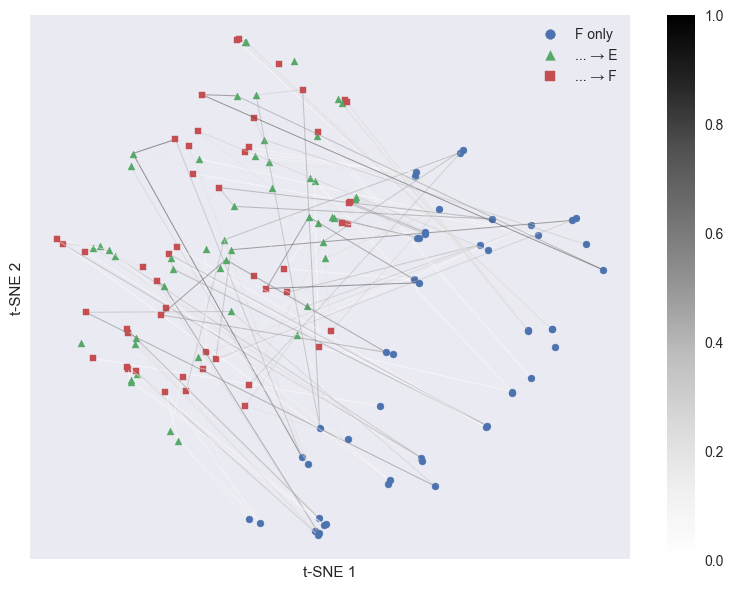
\includegraphics[width=\textwidth]{images/preliminary/tsne-regf-indist-lines.png}
        \caption{Regulation \textbf{F}, in-distribution.}
        \label{fig:tsne-regf-indist-lines}
    \end{subfigure}%
    \begin{subfigure}{.5\textwidth}
        \centering
        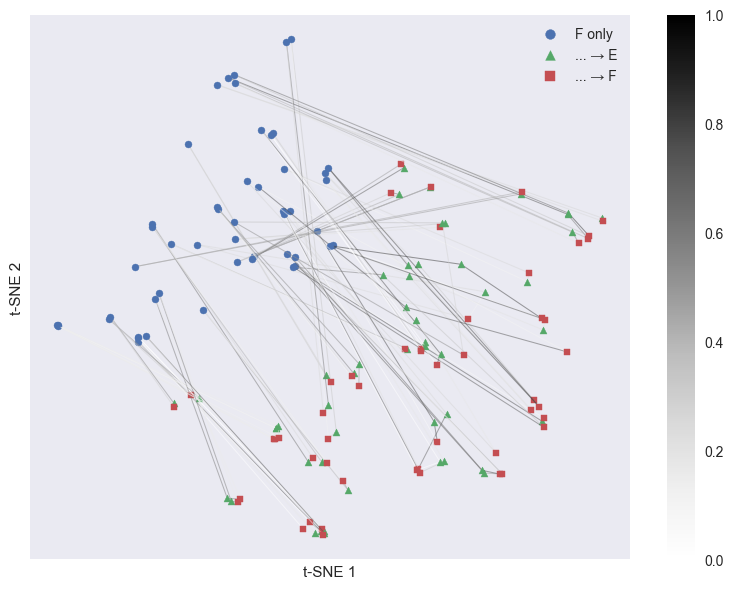
\includegraphics[width=\textwidth]{images/preliminary/tsne-regf-outofdist-lines.png}
        \caption{Regulation \textbf{F}, out-of-distribution.}
        \label{fig:tsne-regf-outdist-lines}
    \end{subfigure}
    \vskip\baselineskip
    \begin{subfigure}{.5\textwidth}
        \centering
        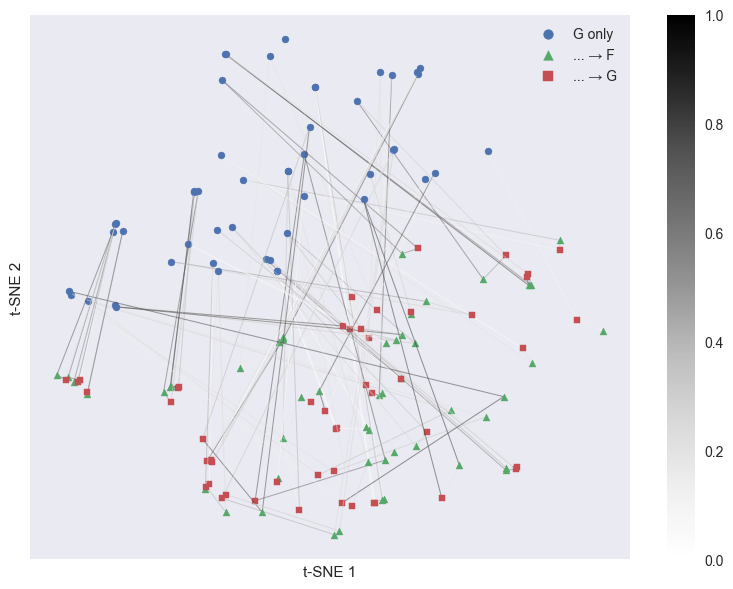
\includegraphics[width=\textwidth]{images/preliminary/tsne-regg-indist-lines.png}
        \caption{Regulation \textbf{G}, in-distribution.}
        \label{fig:tsne-regg-indist-lines}
    \end{subfigure}%
    \begin{subfigure}{.5\textwidth}
        \centering
        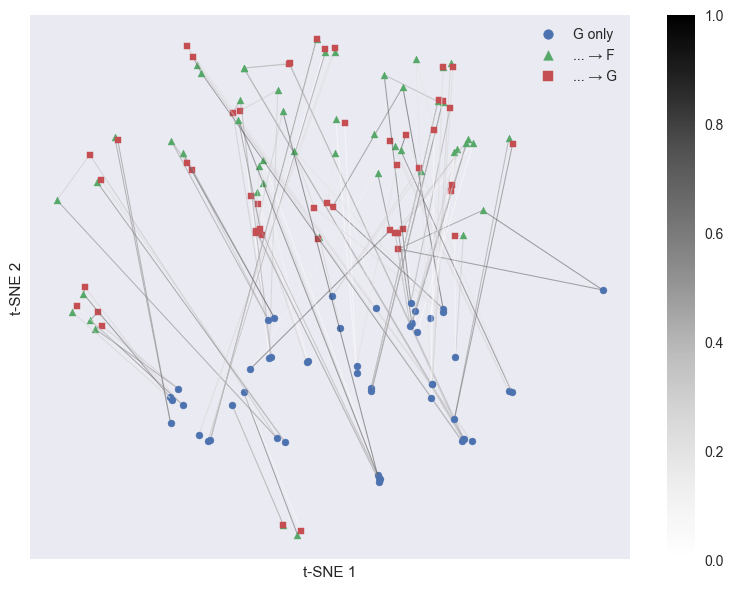
\includegraphics[width=\textwidth]{images/preliminary/tsne-regg-outofdist-lines.png}
        \caption{Regulation \textbf{G}, out-of-distribution.}
        \label{fig:tsne-regg-outdist-lines}
    \end{subfigure}
    \caption{t-SNE visualization of action logits for 50 sampled observations. Letters represent the regulation the agent in trained or fine-tuned on (e.g. ``$... \rightarrow \text{F}$" is fine-tuned from regulation \textbf{A} to \textbf{B} to ... to \textbf{F}). Lines connect points showing the same observation, and are colored according to the Jensen-Shannon distance between the respective action probabilities.}
    \label{fig:tsne-lines}
\end{figure}

Looking closely at Figure \ref{fig:tsne-lines}, we can observe that most of the action logits from the model trained from scratch (the blue circles) have dark lines at narrow, acute angles connecting them to the action logits of the other models.
This suggests that, generally speaking, the action logits and action probabilities of the two fine-tuned models stay closer to each other than to the model trained from scratch.
Similarly to the results shown in Figure \ref{fig:jsd}, this points towards the fine-tuned models potentially suffering from loss of plasticity.

\section{Conclusion} \label{sec:preliminary:conclusion}
Rounding up all the results of these preliminary experiments, we reflect back to the two questions posed at the beginning of this chapter:

\paragraph{1. What effect does non-stationarity have on the performance and generalization of reinforcement learning agents in VGC?}
We showed in Chapter \ref{sec:preliminary:transfer} that reinforcement learning agents are not capable of zero-shot transfer when evaluating using in-distribution teams.
When evaluating for generalization using out-of-distribution teams, the agents are capable of zero-shot transfer to future regulations, though there do exist outliers that will need further investigation.

\paragraph{2. To what extent are reinforcement learning agents able to maintain performance under non-stationarity without any continual learning techniques?}
We showed in Chapter \ref{sec:preliminary:finetune} that, in the best case, full fine-tuning can lead to positive transfer in the short term, but starts to lose out to complete retraining as the game moves further away from its initial definition.
Like before, we also observed multiple outliers here that will need further investigation.

Looking further into the behavior of the fine-tuned models in Chapter \ref{sec:preliminary:analysis}, we saw in Figures \ref{fig:jsd} and \ref{fig:tsne-lines} that the fine-tuned models are potentially held back by a loss of plasticity that causes them to stay too similar to their source model, preventing them from fully adapting to the new regulation.
We also observed unexpected and inconsistent behavior from the value function in Figure \ref{fig:value}, though it is unclear what effect this has on the performance, generalization, and transferability of the model.
We also have to acknowledge here that these experiments were only performed on one seed, making further experimentation necessary.
